
%% bare_conf_compsoc.tex
%% V1.4b
%% 2015/08/26
%% by Michael Shell
%% See:
%% http://www.michaelshell.org/
%% for current contact information.
%%
%% This is a skeleton file demonstrating the use of IEEEtran.cls
%% (requires IEEEtran.cls version 1.8b or later) with an IEEE Computer
%% Society conference paper.
%%
%% Support sites:
%% http://www.michaelshell.org/tex/ieeetran/
%% http://www.ctan.org/pkg/ieeetran
%% and
%% http://www.ieee.org/

%%*************************************************************************
%% Legal Notice:
%% This code is offered as-is without any warranty either expressed or
%% implied; without even the implied warranty of MERCHANTABILITY or
%% FITNESS FOR A PARTICULAR PURPOSE! 
%% User assumes all risk.
%% In no event shall the IEEE or any contributor to this code be liable for
%% any damages or losses, including, but not limited to, incidental,
%% consequential, or any other damages, resulting from the use or misuse
%% of any information contained here.
%%
%% All comments are the opinions of their respective authors and are not
%% necessarily endorsed by the IEEE.
%%
%% This work is distributed under the LaTeX Project Public License (LPPL)
%% ( http://www.latex-project.org/ ) version 1.3, and may be freely used,
%% distributed and modified. A copy of the LPPL, version 1.3, is included
%% in the base LaTeX documentation of all distributions of LaTeX released
%% 2003/12/01 or later.
%% Retain all contribution notices and credits.
%% ** Modified files should be clearly indicated as such, including  **
%% ** renaming them and changing author support contact information. **
%%*************************************************************************


% *** Authors should verify (and, if needed, correct) their LaTeX system  ***
% *** with the testflow diagnostic prior to trusting their LaTeX platform ***
% *** with production work. The IEEE's font choices and paper sizes can   ***
% *** trigger bugs that do not appear when using other class files.       ***                          ***
% The testflow support page is at:
% http://www.michaelshell.org/tex/testflow/



\documentclass[conference,compsoc]{IEEEtran}
% Some/most Computer Society conferences require the compsoc mode option,
% but others may want the standard conference format.
%
% If IEEEtran.cls has not been installed into the LaTeX system files,
% manually specify the path to it like:
% \documentclass[conference,compsoc]{../sty/IEEEtran}





% Some very useful LaTeX packages include:
% (uncomment the ones you want to load)


% *** MISC UTILITY PACKAGES ***
%
%\usepackage{ifpdf}
% Heiko Oberdiek's ifpdf.sty is very useful if you need conditional
% compilation based on whether the output is pdf or dvi.
% usage:
% \ifpdf
%   % pdf code
% \else
%   % dvi code
% \fi
% The latest version of ifpdf.sty can be obtained from:
% http://www.ctan.org/pkg/ifpdf
% Also, note that IEEEtran.cls V1.7 and later provides a builtin
% \ifCLASSINFOpdf conditional that works the same way.
% When switching from latex to pdflatex and vice-versa, the compiler may
% have to be run twice to clear warning/error messages.






% *** CITATION PACKAGES ***
%
\ifCLASSOPTIONcompsoc
  % IEEE Computer Society needs nocompress option
  % requires cite.sty v4.0 or later (November 2003)
  \usepackage[nocompress]{cite}
\else
  % normal IEEE
  \usepackage{cite}
\fi
% cite.sty was written by Donald Arseneau
% V1.6 and later of IEEEtran pre-defines the format of the cite.sty package
% \cite{} output to follow that of the IEEE. Loading the cite package will
% result in citation numbers being automatically sorted and properly
% "compressed/ranged". e.g., [1], [9], [2], [7], [5], [6] without using
% cite.sty will become [1], [2], [5]--[7], [9] using cite.sty. cite.sty's
% \cite will automatically add leading space, if needed. Use cite.sty's
% noadjust option (cite.sty V3.8 and later) if you want to turn this off
% such as if a citation ever needs to be enclosed in parenthesis.
% cite.sty is already installed on most LaTeX systems. Be sure and use
% version 5.0 (2009-03-20) and later if using hyperref.sty.
% The latest version can be obtained at:
% http://www.ctan.org/pkg/cite
% The documentation is contained in the cite.sty file itself.
%
% Note that some packages require special options to format as the Computer
% Society requires. In particular, Computer Society  papers do not use
% compressed citation ranges as is done in typical IEEE papers
% (e.g., [1]-[4]). Instead, they list every citation separately in order
% (e.g., [1], [2], [3], [4]). To get the latter we need to load the cite
% package with the nocompress option which is supported by cite.sty v4.0
% and later.





% *** GRAPHICS RELATED PACKAGES ***
%
\ifCLASSINFOpdf
\usepackage[pdftex]{graphicx}
  % declare the path(s) where your graphic files are
  % \graphicspath{{../pdf/}{../jpeg/}}
  % and their extensions so you won't have to specify these with
  % every instance of \includegraphics
  % \DeclareGraphicsExtensions{.pdf,.jpeg,.png}
\else
  % or other class option (dvipsone, dvipdf, if not using dvips). graphicx
  % will default to the driver specified in the system graphics.cfg if no
  % driver is specified.
  % \usepackage[dvips]{graphicx}
  % declare the path(s) where your graphic files are
  % \graphicspath{{../eps/}}
  % and their extensions so you won't have to specify these with
  % every instance of \includegraphics
  % \DeclareGraphicsExtensions{.eps}
\fi
% graphicx was written by David Carlisle and Sebastian Rahtz. It is
% required if you want graphics, photos, etc. graphicx.sty is already
% installed on most LaTeX systems. The latest version and documentation
% can be obtained at: 
% http://www.ctan.org/pkg/graphicx
% Another good source of documentation is "Using Imported Graphics in
% LaTeX2e" by Keith Reckdahl which can be found at:
% http://www.ctan.org/pkg/epslatex
%
% latex, and pdflatex in dvi mode, support graphics in encapsulated
% postscript (.eps) format. pdflatex in pdf mode supports graphics
% in .pdf, .jpeg, .png and .mps (metapost) formats. Users should ensure
% that all non-photo figures use a vector format (.eps, .pdf, .mps) and
% not a bitmapped formats (.jpeg, .png). The IEEE frowns on bitmapped formats
% which can result in "jaggedy"/blurry rendering of lines and letters as
% well as large increases in file sizes.
%
% You can find documentation about the pdfTeX application at:
% http://www.tug.org/applications/pdftex





% *** MATH PACKAGES ***
%
%\usepackage{amsmath}
% A popular package from the American Mathematical Society that provides
% many useful and powerful commands for dealing with mathematics.
%
% Note that the amsmath package sets \interdisplaylinepenalty to 10000
% thus preventing page breaks from occurring within multiline equations. Use:
%\interdisplaylinepenalty=2500
% after loading amsmath to restore such page breaks as IEEEtran.cls normally
% does. amsmath.sty is already installed on most LaTeX systems. The latest
% version and documentation can be obtained at:
% http://www.ctan.org/pkg/amsmath





% *** SPECIALIZED LIST PACKAGES ***
%
%\usepackage{algorithmic}
% algorithmic.sty was written by Peter Williams and Rogerio Brito.
% This package provides an algorithmic environment fo describing algorithms.
% You can use the algorithmic environment in-text or within a figure
% environment to provide for a floating algorithm. Do NOT use the algorithm
% floating environment provided by algorithm.sty (by the same authors) or
% algorithm2e.sty (by Christophe Fiorio) as the IEEE does not use dedicated
% algorithm float types and packages that provide these will not provide
% correct IEEE style captions. The latest version and documentation of
% algorithmic.sty can be obtained at:
% http://www.ctan.org/pkg/algorithms
% Also of interest may be the (relatively newer and more customizable)
% algorithmicx.sty package by Szasz Janos:
% http://www.ctan.org/pkg/algorithmicx




% *** ALIGNMENT PACKAGES ***
%
%\usepackage{array}
% Frank Mittelbach's and David Carlisle's array.sty patches and improves
% the standard LaTeX2e array and tabular environments to provide better
% appearance and additional user controls. As the default LaTeX2e table
% generation code is lacking to the point of almost being broken with
% respect to the quality of the end results, all users are strongly
% advised to use an enhanced (at the very least that provided by array.sty)
% set of table tools. array.sty is already installed on most systems. The
% latest version and documentation can be obtained at:
% http://www.ctan.org/pkg/array


% IEEEtran contains the IEEEeqnarray family of commands that can be used to
% generate multiline equations as well as matrices, tables, etc., of high
% quality.




% *** SUBFIGURE PACKAGES ***
%\ifCLASSOPTIONcompsoc
%  \usepackage[caption=false,font=footnotesize,labelfont=sf,textfont=sf]{subfig}
%\else
%  \usepackage[caption=false,font=footnotesize]{subfig}
%\fi
% subfig.sty, written by Steven Douglas Cochran, is the modern replacement
% for subfigure.sty, the latter of which is no longer maintained and is
% incompatible with some LaTeX packages including fixltx2e. However,
% subfig.sty requires and automatically loads Axel Sommerfeldt's caption.sty
% which will override IEEEtran.cls' handling of captions and this will result
% in non-IEEE style figure/table captions. To prevent this problem, be sure
% and invoke subfig.sty's "caption=false" package option (available since
% subfig.sty version 1.3, 2005/06/28) as this is will preserve IEEEtran.cls
% handling of captions.
% Note that the Computer Society format requires a sans serif font rather
% than the serif font used in traditional IEEE formatting and thus the need
% to invoke different subfig.sty package options depending on whether
% compsoc mode has been enabled.
%
% The latest version and documentation of subfig.sty can be obtained at:
% http://www.ctan.org/pkg/subfig




% *** FLOAT PACKAGES ***
%
%\usepackage{fixltx2e}
% fixltx2e, the successor to the earlier fix2col.sty, was written by
% Frank Mittelbach and David Carlisle. This package corrects a few problems
% in the LaTeX2e kernel, the most notable of which is that in current
% LaTeX2e releases, the ordering of single and double column floats is not
% guaranteed to be preserved. Thus, an unpatched LaTeX2e can allow a
% single column figure to be placed prior to an earlier double column
% figure.
% Be aware that LaTeX2e kernels dated 2015 and later have fixltx2e.sty's
% corrections already built into the system in which case a warning will
% be issued if an attempt is made to load fixltx2e.sty as it is no longer
% needed.
% The latest version and documentation can be found at:
% http://www.ctan.org/pkg/fixltx2e


%\usepackage{stfloats}
% stfloats.sty was written by Sigitas Tolusis. This package gives LaTeX2e
% the ability to do double column floats at the bottom of the page as well
% as the top. (e.g., "\begin{figure*}[!b]" is not normally possible in
% LaTeX2e). It also provides a command:
%\fnbelowfloat
% to enable the placement of footnotes below bottom floats (the standard
% LaTeX2e kernel puts them above bottom floats). This is an invasive package
% which rewrites many portions of the LaTeX2e float routines. It may not work
% with other packages that modify the LaTeX2e float routines. The latest
% version and documentation can be obtained at:
% http://www.ctan.org/pkg/stfloats
% Do not use the stfloats baselinefloat ability as the IEEE does not allow
% \baselineskip to stretch. Authors submitting work to the IEEE should note
% that the IEEE rarely uses double column equations and that authors should try
% to avoid such use. Do not be tempted to use the cuted.sty or midfloat.sty
% packages (also by Sigitas Tolusis) as the IEEE does not format its papers in
% such ways.
% Do not attempt to use stfloats with fixltx2e as they are incompatible.
% Instead, use Morten Hogholm'a dblfloatfix which combines the features
% of both fixltx2e and stfloats:
%
% \usepackage{dblfloatfix}
% The latest version can be found at:
% http://www.ctan.org/pkg/dblfloatfix




% *** PDF, URL AND HYPERLINK PACKAGES ***
%
%\usepackage{url}
% url.sty was written by Donald Arseneau. It provides better support for
% handling and breaking URLs. url.sty is already installed on most LaTeX
% systems. The latest version and documentation can be obtained at:
% http://www.ctan.org/pkg/url
% Basically, \url{my_url_here}.




% *** Do not adjust lengths that control margins, column widths, etc. ***
% *** Do not use packages that alter fonts (such as pslatex).         ***
% There should be no need to do such things with IEEEtran.cls V1.6 and later.
% (Unless specifically asked to do so by the journal or conference you plan
% to submit to, of course. )


% correct bad hyphenation here
\hyphenation{op-tical net-works semi-conduc-tor}


\begin{document}
%
% paper title
% Titles are generally capitalized except for words such as a, an, and, as,
% at, but, by, for, in, nor, of, on, or, the, to and up, which are usually
% not capitalized unless they are the first or last word of the title.
% Linebreaks \\ can be used within to get better formatting as desired.
% Do not put math or special symbols in the title.
\title{Blockchain and Bitcoin}


% author names and affiliations
% use a multiple column layout for up to three different
% affiliations
\author{\IEEEauthorblockN{Daniyar Jakupov}
\IEEEauthorblockA{INFOTECH\\
3212507\\
University of Stuttgart\\
Stuttgart, Germany\\
Email: drjakupov@gmail.com}
}

% conference papers do not typically use \thanks and this command
% is locked out in conference mode. If really needed, such as for
% the acknowledgment of grants, issue a \IEEEoverridecommandlockouts
% after \documentclass

% for over three affiliations, or if they all won't fit within the width
% of the page (and note that there is less available width in this regard for
% compsoc conferences compared to traditional conferences), use this
% alternative format:
% 
%\author{\IEEEauthorblockN{Michael Shell\IEEEauthorrefmark{1},
%Homer Simpson\IEEEauthorrefmark{2},
%James Kirk\IEEEauthorrefmark{3}, 
%Montgomery Scott\IEEEauthorrefmark{3} and
%Eldon Tyrell\IEEEauthorrefmark{4}}
%\IEEEauthorblockA{\IEEEauthorrefmark{1}School of Electrical and Computer Engineering\\
%Georgia Institute of Technology,
%Atlanta, Georgia 30332--0250\\ Email: see http://www.michaelshell.org/contact.html}
%\IEEEauthorblockA{\IEEEauthorrefmark{2}Twentieth Century Fox, Springfield, USA\\
%Email: homer@thesimpsons.com}
%\IEEEauthorblockA{\IEEEauthorrefmark{3}Starfleet Academy, San Francisco, California 96678-2391\\
%Telephone: (800) 555--1212, Fax: (888) 555--1212}
%\IEEEauthorblockA{\IEEEauthorrefmark{4}Tyrell Inc., 123 Replicant Street, Los Angeles, California 90210--4321}}




% use for special paper notices
%\IEEEspecialpapernotice{(Invited Paper)}




% make the title area
\maketitle

% As a general rule, do not put math, special symbols or citations
% in the abstract
\begin{abstract}
Bitcoin emerged as an alternative to traditional fiat currencies in 2008 and gained its value among established financial institutions in a span of several years. The concept behind it relies on blockchain technology which can be described as a public system of decentralized trustless verification based on mathematical cryptography. In other words, bitcoin is distributed digital ledger that lists financial transaction. 


\end{abstract}

% no keywords




% For peer review papers, you can put extra information on the cover
% page as needed:
% \ifCLASSOPTIONpeerreview
% \begin{center} \bfseries EDICS Category: 3-BBND \end{center}
% \fi
%
% For peerreview papers, this IEEEtran command inserts a page break and
% creates the second title. It will be ignored for other modes.
\IEEEpeerreviewmaketitle



\section{Introduction}
% no \IEEEPARstart
In this paper, we discuss various topics related to blockchain technology and bitcoin itself. Firstly, we start with the history of digital currencies and why bitcoin was the first one to succeed. It leads us to principles of blockchain technology and why it was used for bitcoin. Then we look under the hood and learn how bitcoin works in real world. Finally, we examine different areas where blockchain is used on its own without bitcoin. We conclude by summarizing what we learned and what could be the future of these technologies.
% You must have at least 2 lines in the paragraph with the drop letter
% (should never be an issue)


% An example of a floating figure using the graphicx package.
% Note that \label must occur AFTER (or within) \caption.
% For figures, \caption should occur after the \includegraphics.
% Note that IEEEtran v1.7 and later has special internal code that
% is designed to preserve the operation of \label within \caption
% even when the captionsoff option is in effect. However, because
% of issues like this, it may be the safest practice to put all your
% \label just after \caption rather than within \caption{}.
%
% Reminder: the "draftcls" or "draftclsnofoot", not "draft", class
% option should be used if it is desired that the figures are to be
% displayed while in draft mode.
%
%\begin{figure}[!t]
%\centering
%\includegraphics[width=2.5in]{myfigure}
% where an .eps filename suffix will be assumed under latex, 
% and a .pdf suffix will be assumed for pdflatex; or what has been declared
% via \DeclareGraphicsExtensions.
%\caption{Simulation results for the network.}
%\label{fig_sim}
%\end{figure}

% Note that the IEEE typically puts floats only at the top, even when this
% results in a large percentage of a column being occupied by floats.


% An example of a double column floating figure using two subfigures.
% (The subfig.sty package must be loaded for this to work.)
% The subfigure \label commands are set within each subfloat command,
% and the \label for the overall figure must come after \caption.
% \hfil is used as a separator to get equal spacing.
% Watch out that the combined width of all the subfigures on a 
% line do not exceed the text width or a line break will occur.
%
%\begin{figure*}[!t]
%\centering
%\subfloat[Case I]{\includegraphics[width=2.5in]{box}%
%\label{fig_first_case}}
%\hfil
%\subfloat[Case II]{\includegraphics[width=2.5in]{box}%
%\label{fig_second_case}}
%\caption{Simulation results for the network.}
%\label{fig_sim}
%\end{figure*}
%
% Note that often IEEE papers with subfigures do not employ subfigure
% captions (using the optional argument to \subfloat[]), but instead will
% reference/describe all of them (a), (b), etc., within the main caption.
% Be aware that for subfig.sty to generate the (a), (b), etc., subfigure
% labels, the optional argument to \subfloat must be present. If a
% subcaption is not desired, just leave its contents blank,
% e.g., \subfloat[].


% An example of a floating table. Note that, for IEEE style tables, the
% \caption command should come BEFORE the table and, given that table
% captions serve much like titles, are usually capitalized except for words
% such as a, an, and, as, at, but, by, for, in, nor, of, on, or, the, to
% and up, which are usually not capitalized unless they are the first or
% last word of the caption. Table text will default to \footnotesize as
% the IEEE normally uses this smaller font for tables.
% The \label must come after \caption as always.
%
%\begin{table}[!t]
%% increase table row spacing, adjust to taste
%\renewcommand{\arraystretch}{1.3}
% if using array.sty, it might be a good idea to tweak the value of
% \extrarowheight as needed to properly center the text within the cells
%\caption{An Example of a Table}
%\label{table_example}
%\centering
%% Some packages, such as MDW tools, offer better commands for making tables
%% than the plain LaTeX2e tabular which is used here.
%\begin{tabular}{|c||c|}
%\hline
%One & Two\\
%\hline
%Three & Four\\
%\hline
%\end{tabular}
%\end{table}


% Note that the IEEE does not put floats in the very first column
% - or typically anywhere on the first page for that matter. Also,
% in-text middle ("here") positioning is typically not used, but it
% is allowed and encouraged for Computer Society conferences (but
% not Computer Society journals). Most IEEE journals/conferences use
% top floats exclusively. 
% Note that, LaTeX2e, unlike IEEE journals/conferences, places
% footnotes above bottom floats. This can be corrected via the
% \fnbelowfloat command of the stfloats package.


\section{Main Part}

\subsection{History of digital currencies}
Ever since internet starts to gain its popularity among the masses, people were thinking on how to adapt traditional financial system to digital world. 
One of the pioneers in this area were three enthusiasts, namely Eric Hughes, mathematician from University of California, Berkeley; Tim May, senior scientist at Intel and John Gilmore a computer scientist from Sun Microsystems. 
In 1992 they organized a group called Cypherpunks in Bay Area with the goal of adapting traditional monetary system to digital society where privacy will be guaranteed with the help of programming and cryptography. 
This underlying principle is highlighted in their manifesto [1].
Quickly, this group became popular and people were joining it all across the globe through its encrypted and anonymous mailing list, which was one of the first in a world. 
As a result of this discussions, many of its members proposed various solutions for creation of digital currency which later would become foundations for the development of Bitcoin. 
So let us examine some proposals published by members of Cypherpunk mailing list.

\subsubsection{Early attempts}
We start in 1997 with Dr. Adam Back who developed a system for preventing digital spamming called Hashcash [2]. 
He was one of the first to use Proof-of-Work (PoW) algorithm in real application by forcing users to spend computational power on a creation of a hash that is included in email header. 
This hash is easily verifiable, but impossible to hack using brute-force. 
This serves as a proof that certain amount of time was spend to create an email, thus making spamming inefficient. 
Later, we examine how this algorithm is used in Bitcoin. 

One year later, Wei Dai, a computer engineer, published a proposal for "b-money, an anonymous, distributed electronic cash system" [3]. He developed two protocols that could be used in such cash system. First protocol requires every user of the network to keep separate database of all transactions. Money creation happens by solving computational problems and money transfer occurs by broadcasting transaction details to all participants. You may notice that this protocol is using PoW concept. Second protocol has a different approach to transaction storage. Instead of using every member of network to keep database, only subset of participants is responsible for verification of transactions. To ensure that such users will be honest, they are required to deposit their own funds in special account in case of a fraudulent behavior. This protocol later will be known as Proof-of-Stake (PoS). Nowadays, many cryptocurrencies are using this method. 

In 2004, Hal Finney, a computer scientist, creates so called Reusable Proof of Work (RPOW) tokens that can be used in a form of digital cash [4]. 
The system consist of three parts: client, host, and server. Each has its own responsibilities. 
The interesting part of this software is that tokens are completely unique, but also have limited re-usability quality, thus preventing double spending, which is one of the fundamental problems of digital cash. 

In 2005, Nick Szabo, computer scientist and cryptographer, republishes his proposal from 1998 called Bitgold. 
There he describes a system that works as decentralized digital currency, similar to RPOW system by Hal Finney. 
The difference is that PoW in RPOW relies upon specific computer architecture, which can be leveraged at some point in time, whereas Bitgold uses additional timestamps by implementing linked structure for transactions, thus making it possible to proof mathematical difficulty of the work at any moment in history. 
Unfortunately, Bitgold was only implemented on paper.

Here we examined just some attempts to develop fully functional digital currency. 
There were many more, but for one reason or another, none of them were successful. 
At least, not until year 2008. 

\subsubsection{Pros and cons of digital currency}
What makes digital currency creation so hard? There are two main problems that need to be solved. 
First one is how to ensure that money spend belongs to a certain user without revealing how to access them. 
Second problem is a possibility to spend one digital token multiple times by copying it to a point where counterfeits are indistinguishable and using network latency during the sending process. 
Because of that, creation of fully independent and distributed digital currency was not done for a long time. 

However, after financial crisis in 2008 which caused millions of people around the world to loose their homes and jobs and additionally tanking major global economies such as USA and EU [5].
As a consequence, interest in alternative ways of doing financial operations outside of traditional banking system was rekindled. 
In addition, people already knew what kind of advantages digital currency could bring. Here are some examples:
\begin{itemize}
  \item Easy accounting and access. 
  \item International. 
  \item Cheap. 
  \item Internet ready
\end{itemize}

\subsection{Blockchain: blueprint for Bitcoin}
Coincidentally, in October of 2008 someone releases a paper addressing this issue. 
The paper was distributed through Cypherpunks mailing list and is called "Bitcoin: A Peer-to-Peer Electronic Cash System" [6]. 
It describes a solution to two problems of digital currencies and allowing to send electronic transactions without relying on trust provided from a third party. 
We do not know who is the author behind this paper. 
Whether it is one person or a group of individuals, we only know the pseudonym which is Satoshi Nakamoto.    

In order to create functional digital currency, Satoshi Nakamoto used technologies that have been developed in a past. 
He started with technology that proved to be working without relying on centralized authority.    
BitTorrent - protocol for decentralized distribution of files was responsible for approximately half of all internet traffic in 2008 [7]. 
Satoshi applied BitTorrent principle to a bank, by taking its centralized part, namely ledger and distributing it across the network. 
To make such distributed ledger work, he applied two technologies: PoW algorithm and elliptic curve digital signature (ECDS) algorithm.
Former solves double-spending problem as we have already seen in previous works whereas latter ensures that funds can be spent only by their rightful owner.
By combining these algorithms together, one can build a decentralized network of trustless verification also known as blockchain. 

\subsection{Bitcoin: under the hood}
There is no single definition for Bitcoin.
But we can characterize it as a digital ledger that lists financial transactions and is distributed across blockchain network. 
From original white paper we know how this network organized: 

\begin{itemize}
  \item Transactions are grouped together into blocks 
  \item Maximum number of transactions per block is ~2600. 
  \item New block is generated every ~10 minutes.
\end{itemize}

As it can be seen on Figure 1 each block is linked to previous block by using its hashed version. 

\begin{figure}[h!]
  \centering
  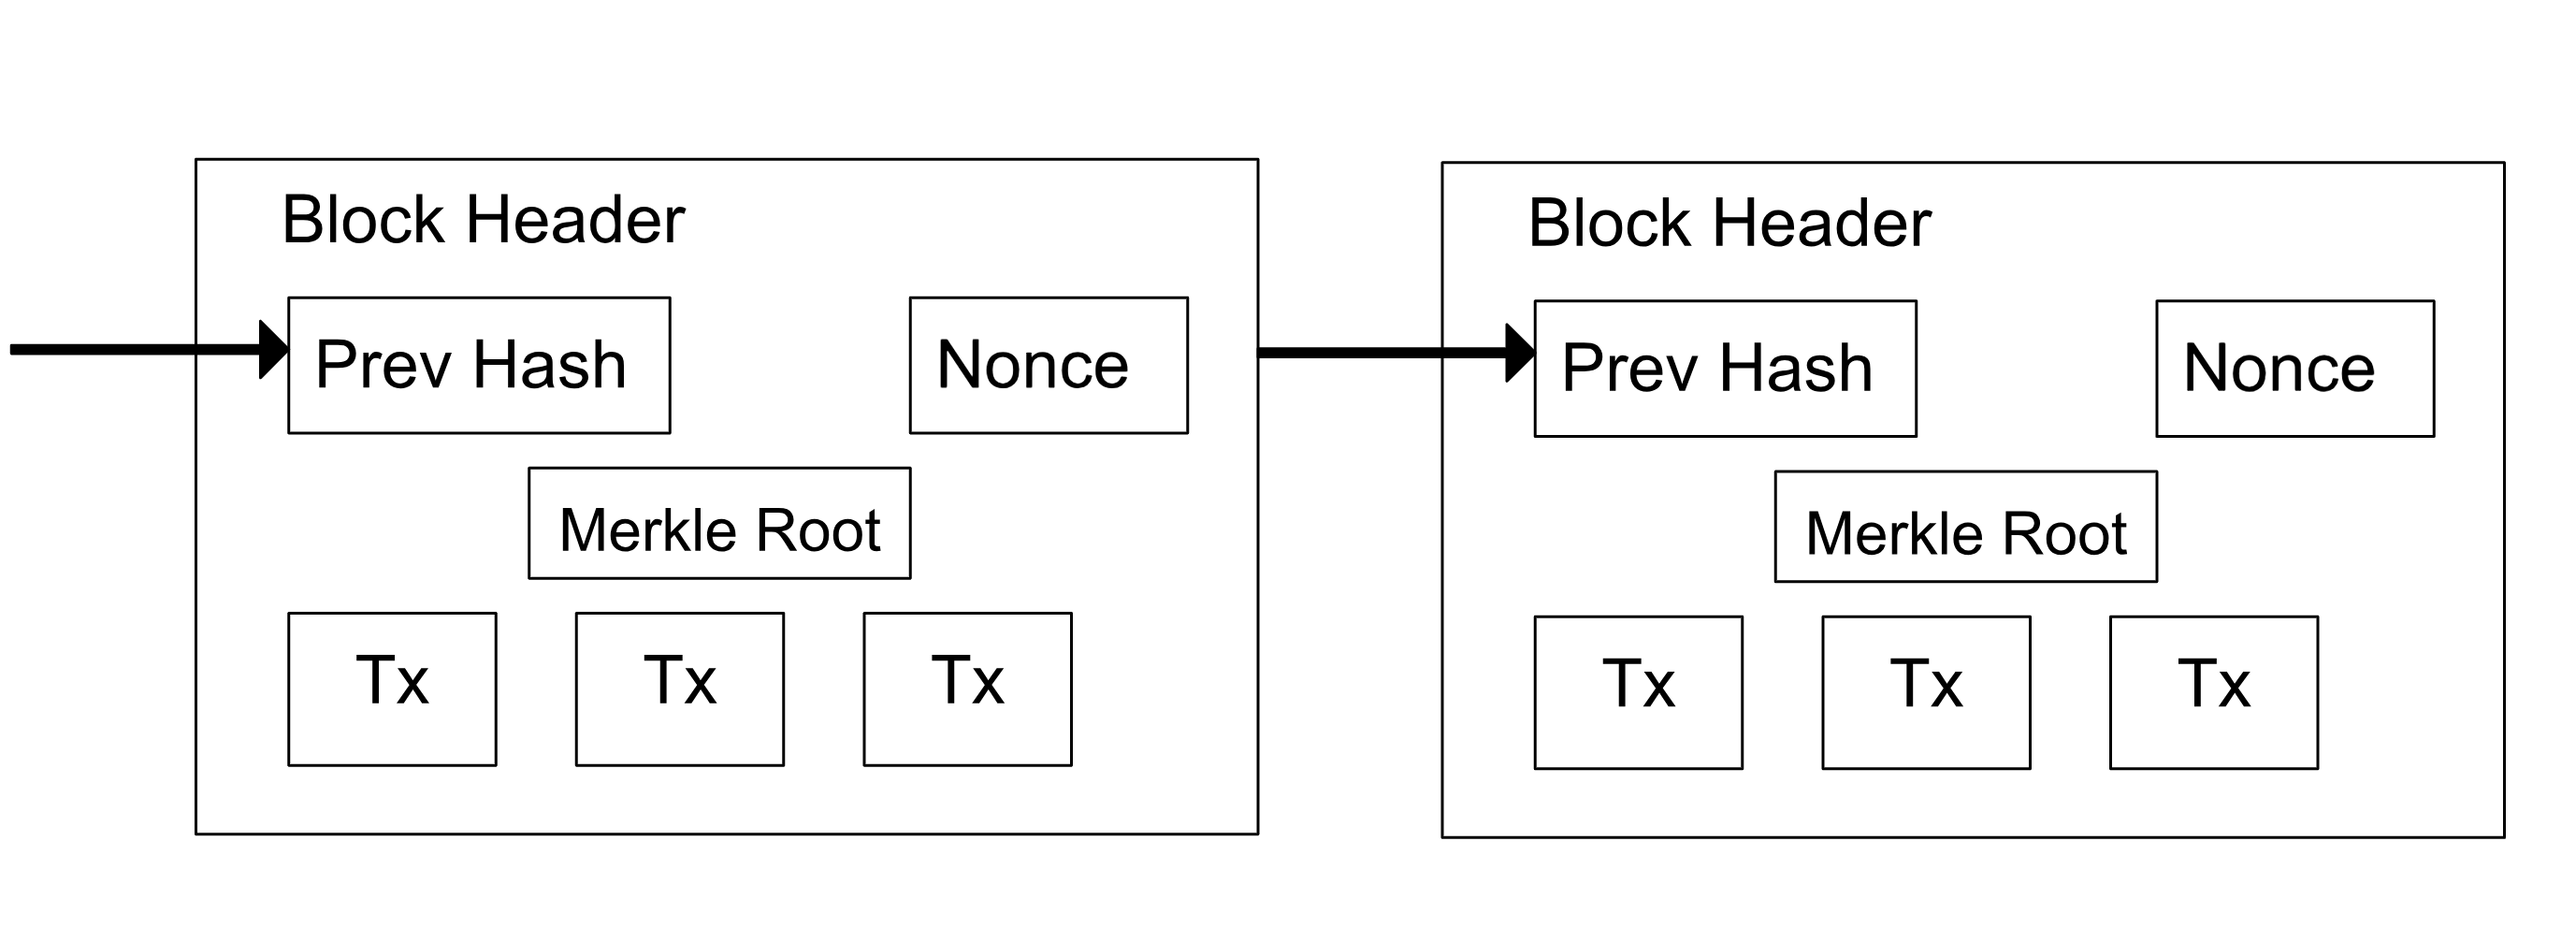
\includegraphics[width=.45\textwidth]{graphics/blocks.png}
  \caption{Bitcoin blocks with transactions}
  \label{fig:fig1}
\end{figure}

\subsubsection{Elliptic Curve Digital Signature}
ECDS cryptographical algorithm is used by Bitcoin in two cases. 
First one is a creation of a wallet where user can access his/her funds.
In order to create and later access wallet, ECSD generates a private key, which is a number in base58 format. This number represent really large integer, to be more precise it is $2^{256}$ or $10^{168}$. 
For a comparison, according to [8] just to count up to $2^{192}$ we will need constantly harvest energy directly from the sun for thirty two years. 
All this implies, that a brute-force attack to find someone's else private key is simply impossible. 
After creating private key, user can generate corresponding public key, which acts as a wallet address inside Bitcoin network and can be shared with anyone. 
Important point is that it is impossible to reverse engineer ECSD algorithm, in other words one can not get a private key from a public key.
Second case for the use of ECDS is a creation of digital signatures.
To generate it, special ECDS function is used that accepts private key and hashed transaction as an arguments. 
Every time when new transaction is created, it has to include new digital signature.
One can not just copy signature from old transaction and use it again, since each transaction contains unique id which leads to a completely new hash.  
To verify that transaction was generated by a person who claims to be an owner and the content has not been changed after its creation, one need to use provided signature, public key and hashed transaction as an arguments for another ECDS function. 
Verification process is really fast and if everything is in order, it returns true, otherwise false.
The process of using private / public key pair for signing transactions is shown on Figure 2.

\begin{figure}[h]
  \centering
  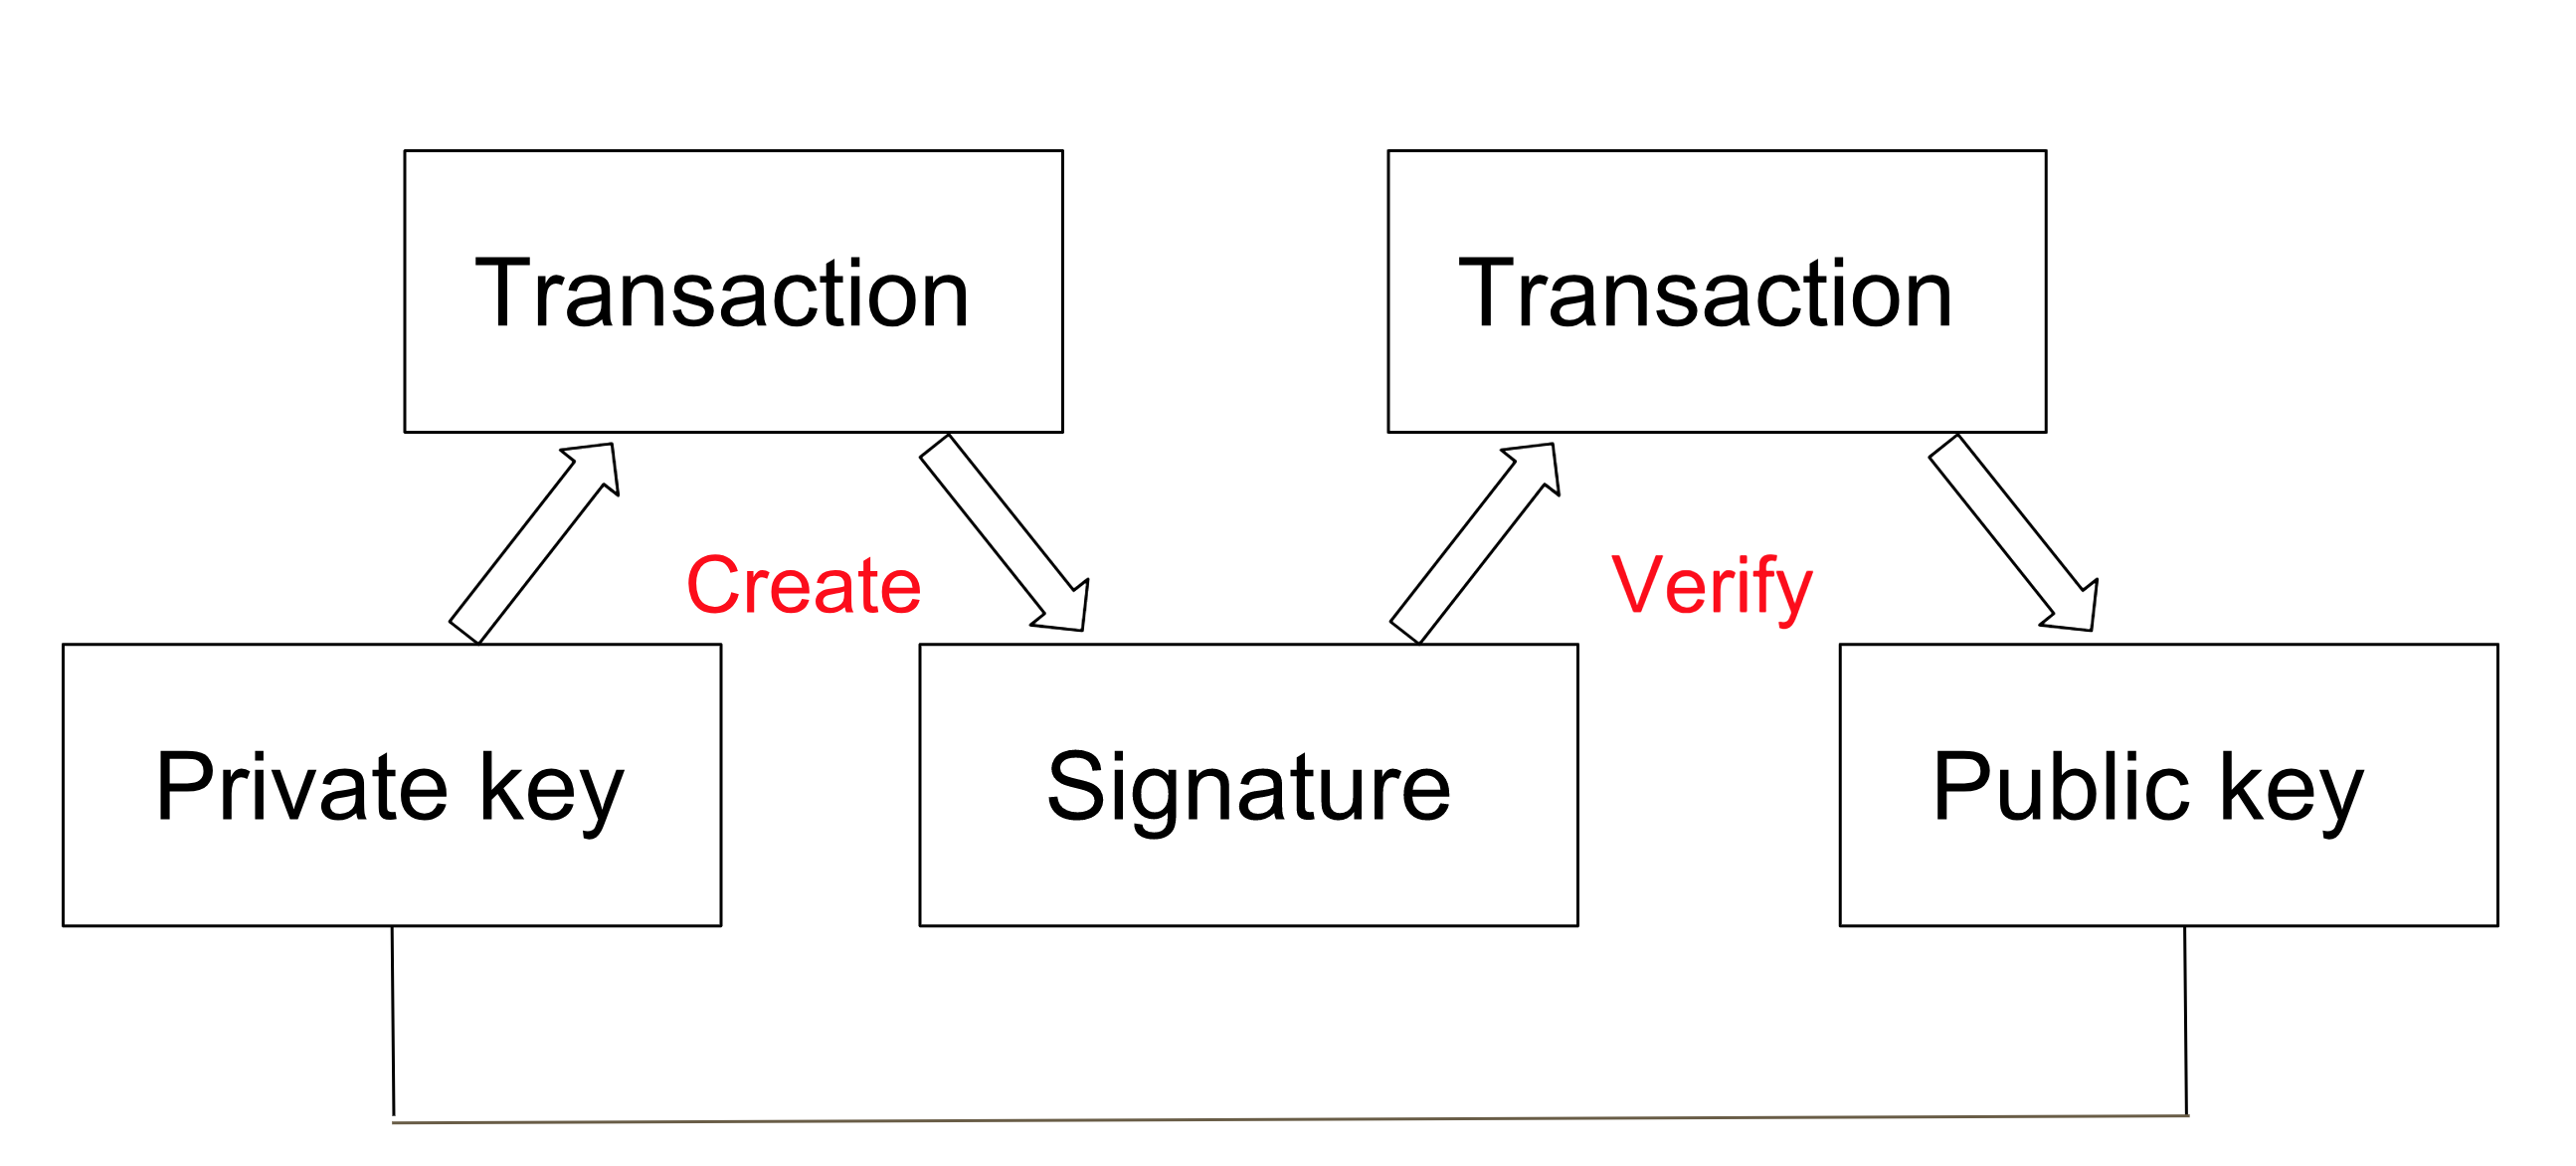
\includegraphics[width=.45\textwidth]{graphics/private_public.png}
  \caption{Signature generation using private / public key pair}
  \label{fig:fig2}
\end{figure}

\subsubsection{Proof Of Work}
Now we can examine how Satoshi Nakamato solved another big problem of digital currencies - double spending.
As we discussed earlier, systems with PoW algorithms already have been developed and tested, such as Dr. Adam Back's Hashcash [2]. 
The underlying principle is to design a system that ensures the right order of transactions. 
We know that transactions are grouped together into blocks and each block has a reference to previous one in a form of its hash. 
But how are blocks generated and what if two blocks arrive at the same time? 

On Figure 1 you might notice special field inside each block called nonce. 
In order to create valid block that could be accepted into Bitcoin network, one must use cryptographic hash function SHA256. 
As an arguments, it accepts hashed block and a random number called nonce.
Result of SHA256 is another 32 bit number. 
This number should satisfy current bitcoin target by having certain number of leading zeros. 
The only way to find such nonce for a specific block is by guessing and checking. 
The first node that finds correct nonce broadcasts the block to the network. 

The whole process of guessing the right nonce is called mining and nonce itself serves as a PoW. 
This ensures that blocks are stored in order of their acceptance inside the network.
It could take quite some time to find a nonce for a single node, but since the number of nodes participating in a mining quite large average time is around ten minutes. 
However, since 2008 computational power is increasing both in quality and quantity, so to keep mining time constant, difficulty level is adjusted after every 2016 blocks or approximately every two weeks. 
If we take difficulty value in the beginning of Bitcoin as one, then by the end of February of 2019 it increased in six trillion times [8].
Figure 3 shows how difficulty changes since the beginning.

\begin{figure}[h]
  \centering
  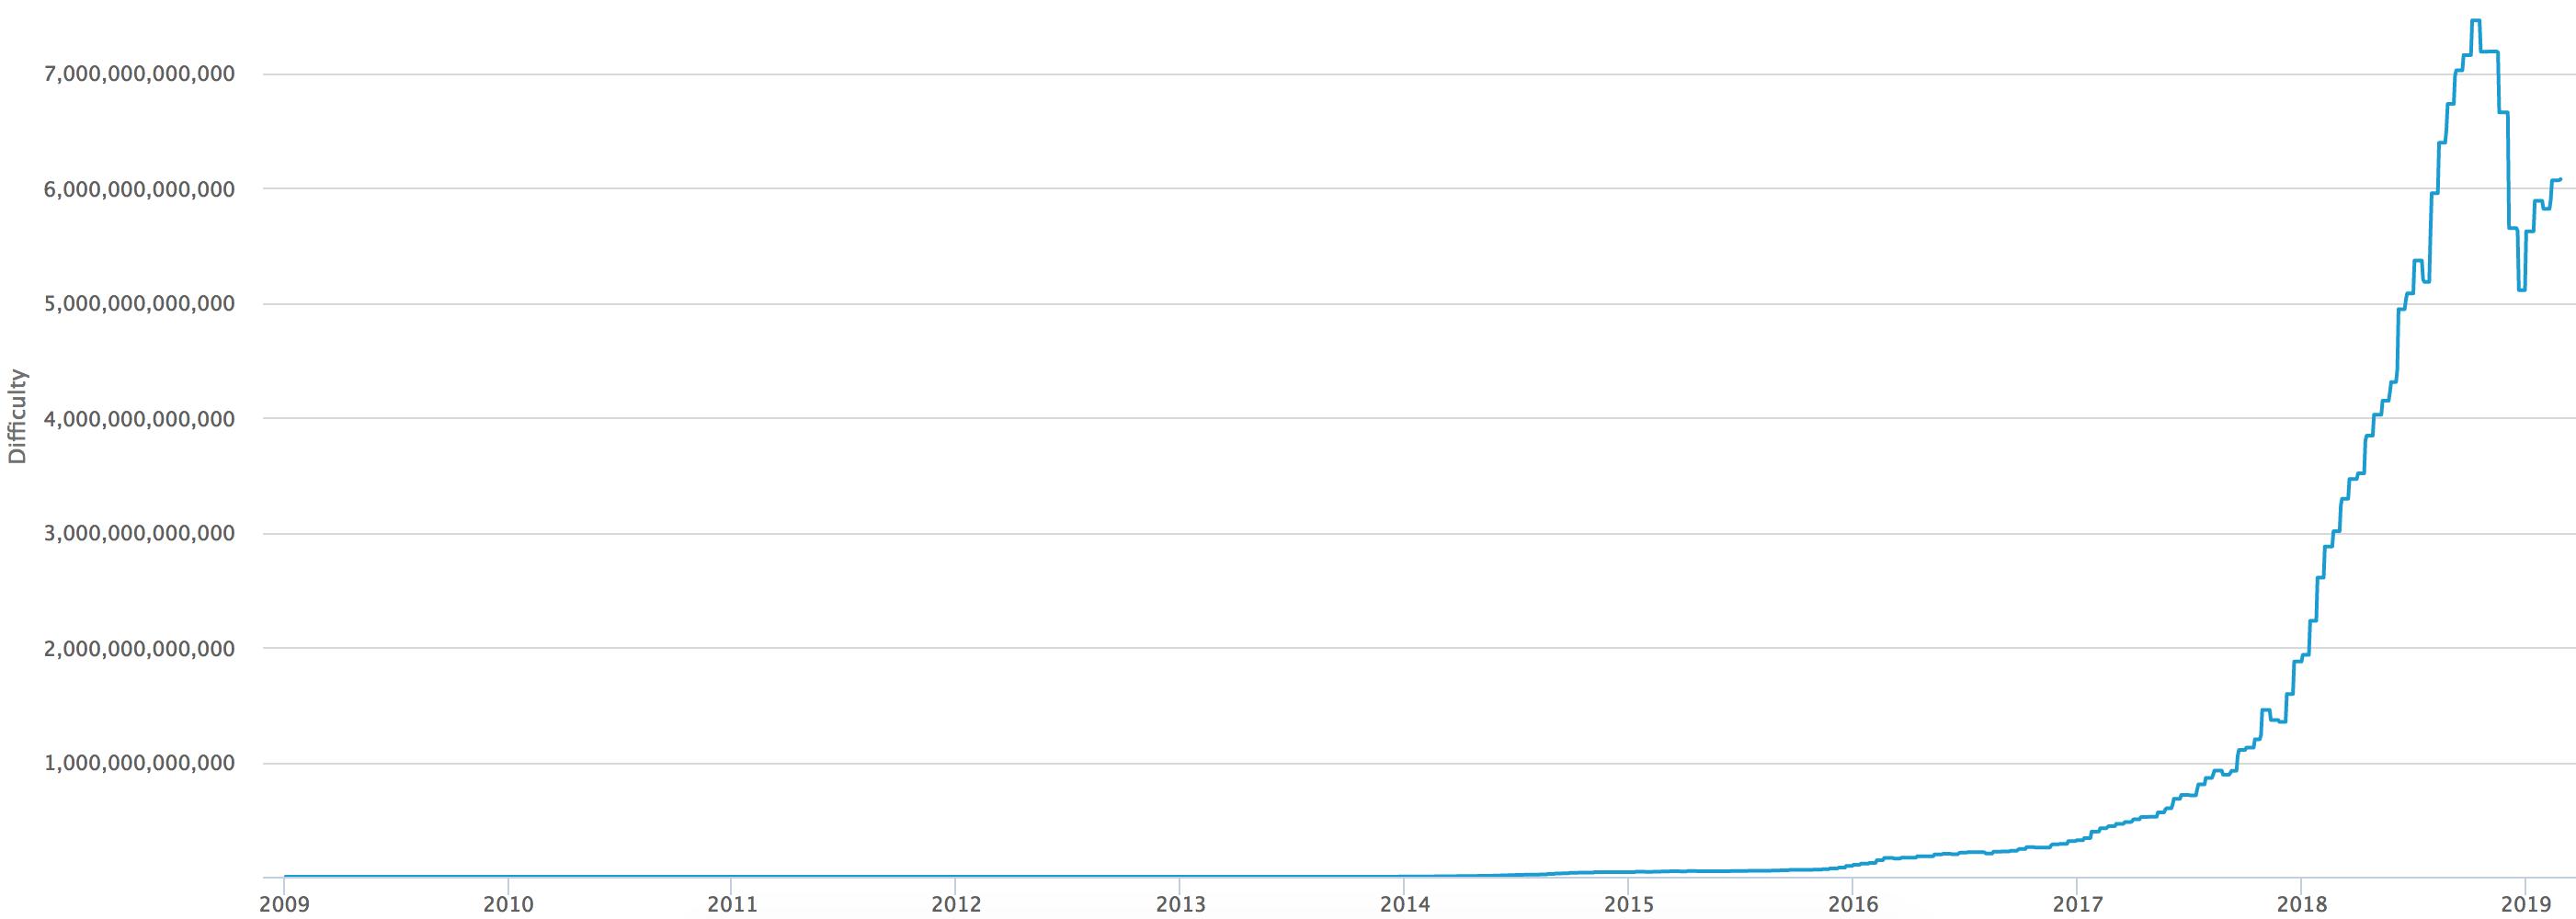
\includegraphics[width=.45\textwidth]{graphics/target.png}
  \caption{Difficulty level}
  \label{fig:fig3}
\end{figure}


Sometimes it can happen, that two nodes solve nonce puzzle at around same time. 
In that case, bitcoin has a protocol that resolves the conflict by creating two branches of a blockchain until one of them becomes longer.
Shorter branch is eliminated and transactions which were grouped in a discarded block will be returned to the pool of unconfirmed transactions.
Thus, it is suggested to wait several blocks to be certain that transaction is recorded in a network.

Attentive reader may notice that above mentioned conflict resolution could be exploited in different double spending attack. 
Here is an example: Alice sends transaction to Bob. 
Bob waits few more blocks to make sure transaction is not dismissed, then ships the product.
Meanwhile, Alice was creating her own version of blockchain, where she send Bob's transaction to herself. 
If Alice is faster in mining new blocks than the rest of network, she can create a longer version of blockchain and announce it to the network, thus uncofirming previous blocks.
Figure 4 illustrates this example.

\begin{figure}[h]
  \centering
  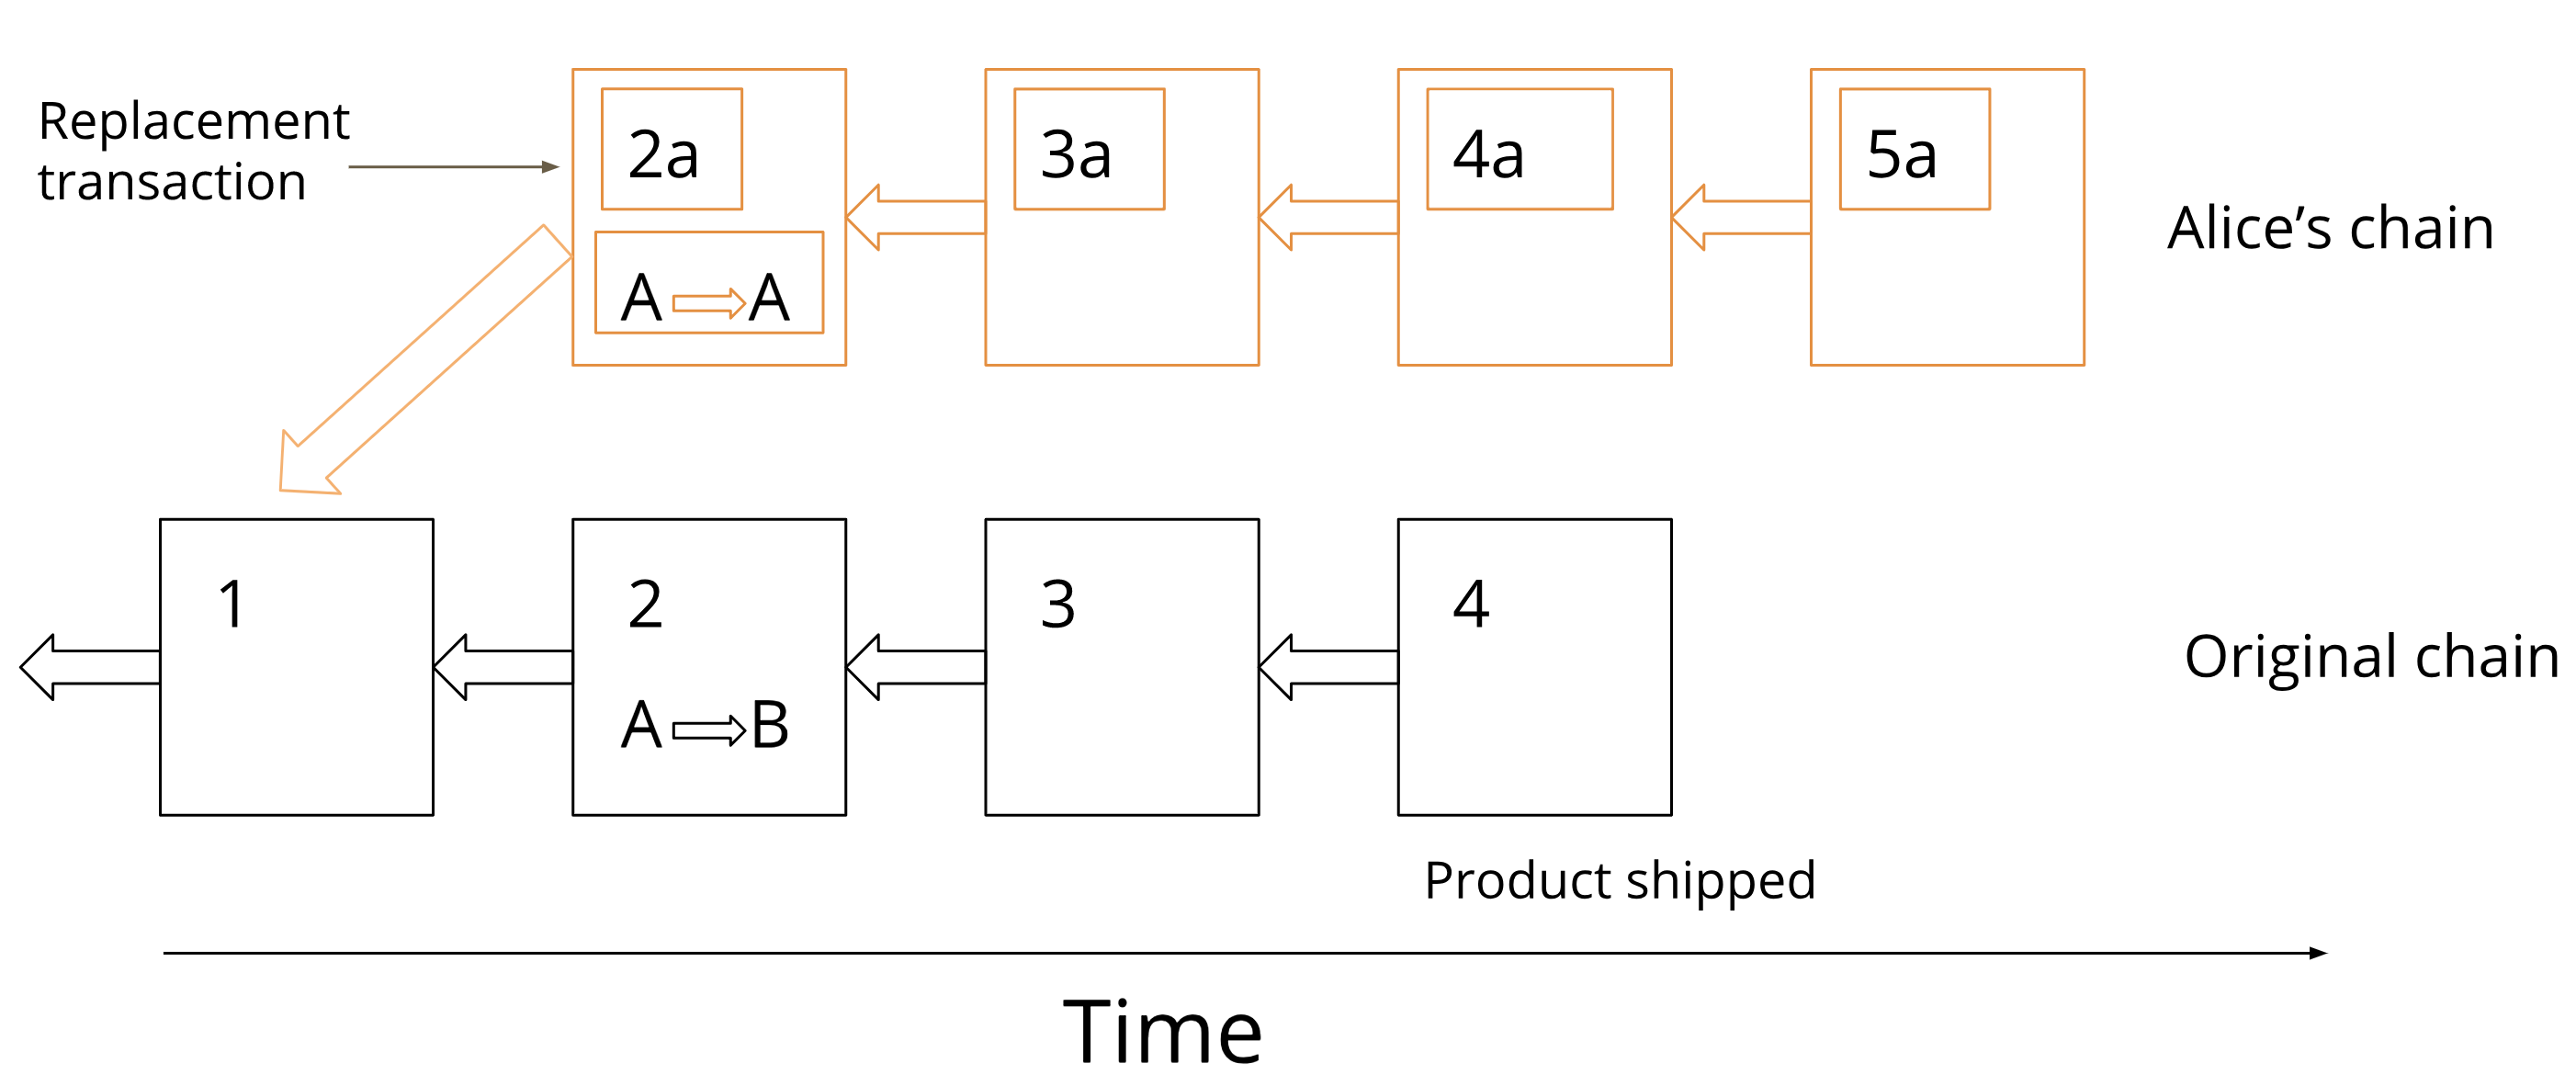
\includegraphics[width=.45\textwidth]{graphics/pow.png}
  \caption{Attack against PoW}
  \label{fig:fig4}
\end{figure}

But can she realistically do such thing? 
Answer is no.
The reason is that she will be trying to outpace the whole network of nodes and as we mentioned the network is creating a new block every ten minutes whereas for individual miner it takes approximately a day. 
It can be compared to a lottery. 
The chances of winning constantly by buying one ticket are close to zero. 
The only way to do it is to have 51\% computational power of the whole network.
This method is called 51\% attack. 
But the only incentive of actually launching such attack is to completely destroy the value of Bitcoin. 

In addition, Alice also cannot just swap one particular block that is already part of a blockchain due to the fact that next block has a reference to it in a form of hash. 
Thus even if one transaction is altered, the whole reference hash becomes invalid and we go back to racing issue.

\subsubsection{Transactions in Bitcoin}
We know that Bitcoin in its simplest definition is a distributed database storing all transactions. 
Transaction consist of at least one input and at most two outputs.
Inputs are needed to reference previous transactions where the sender is recipient and outputs are for specifying public address of a new recipient and for returning the change if needed.
The network will check whether input transactions have been used already, thus verifying that sender has enough funds.
Figure 5 depicts transaction with multiple inputs and two outputs.

\begin{figure}[h]
  \centering
  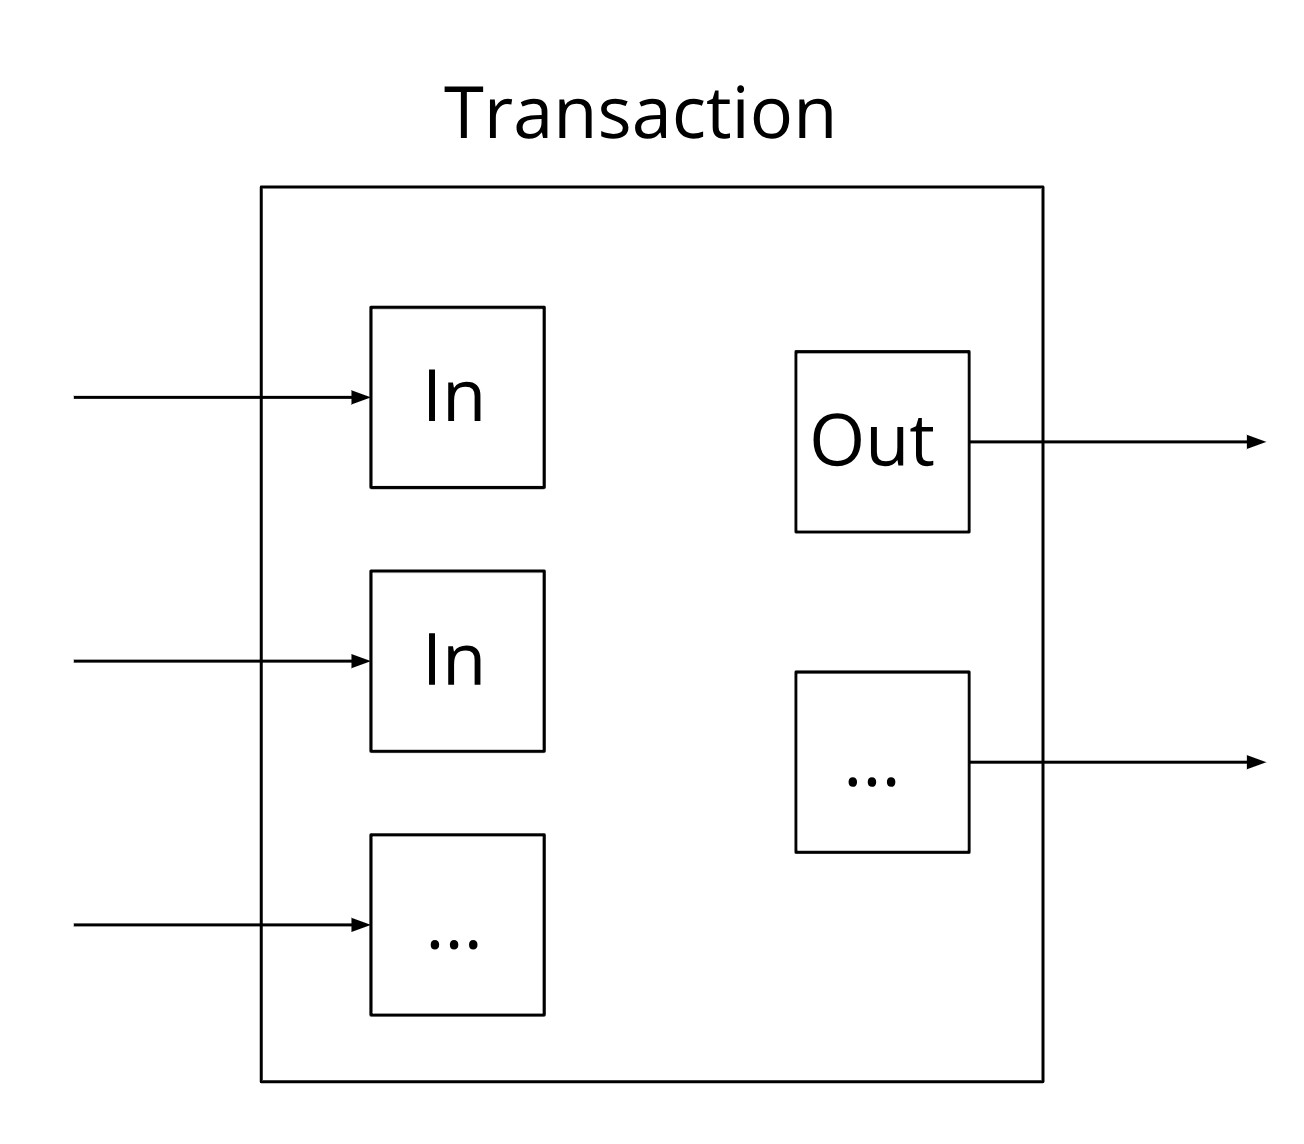
\includegraphics[width=.45\textwidth]{graphics/tx.png}
  \caption{Transaction}
  \label{fig:fig5}
\end{figure}

As it has been already mentioned, each block contains several thousand transactions. 
Visually it can be represented by Figure 1. 

However, in reality Bitcoin network does something different. 
In order to save space by not including the whole transaction body, but keep previous hash inside each block valid, all transaction are hashed in a tree structure called Merkle tree [9].
It works by grouping transactions in pairs and hashing them until one single hash is obtained which is called merkle root. 
If even one of the transactions is altered in any way after Merkle tree is constructed, merkle root will be completely different. 
This root is included in each block.
So, Figure 1 can be adjusted to Figure 6

\begin{figure}[h]
  \centering
  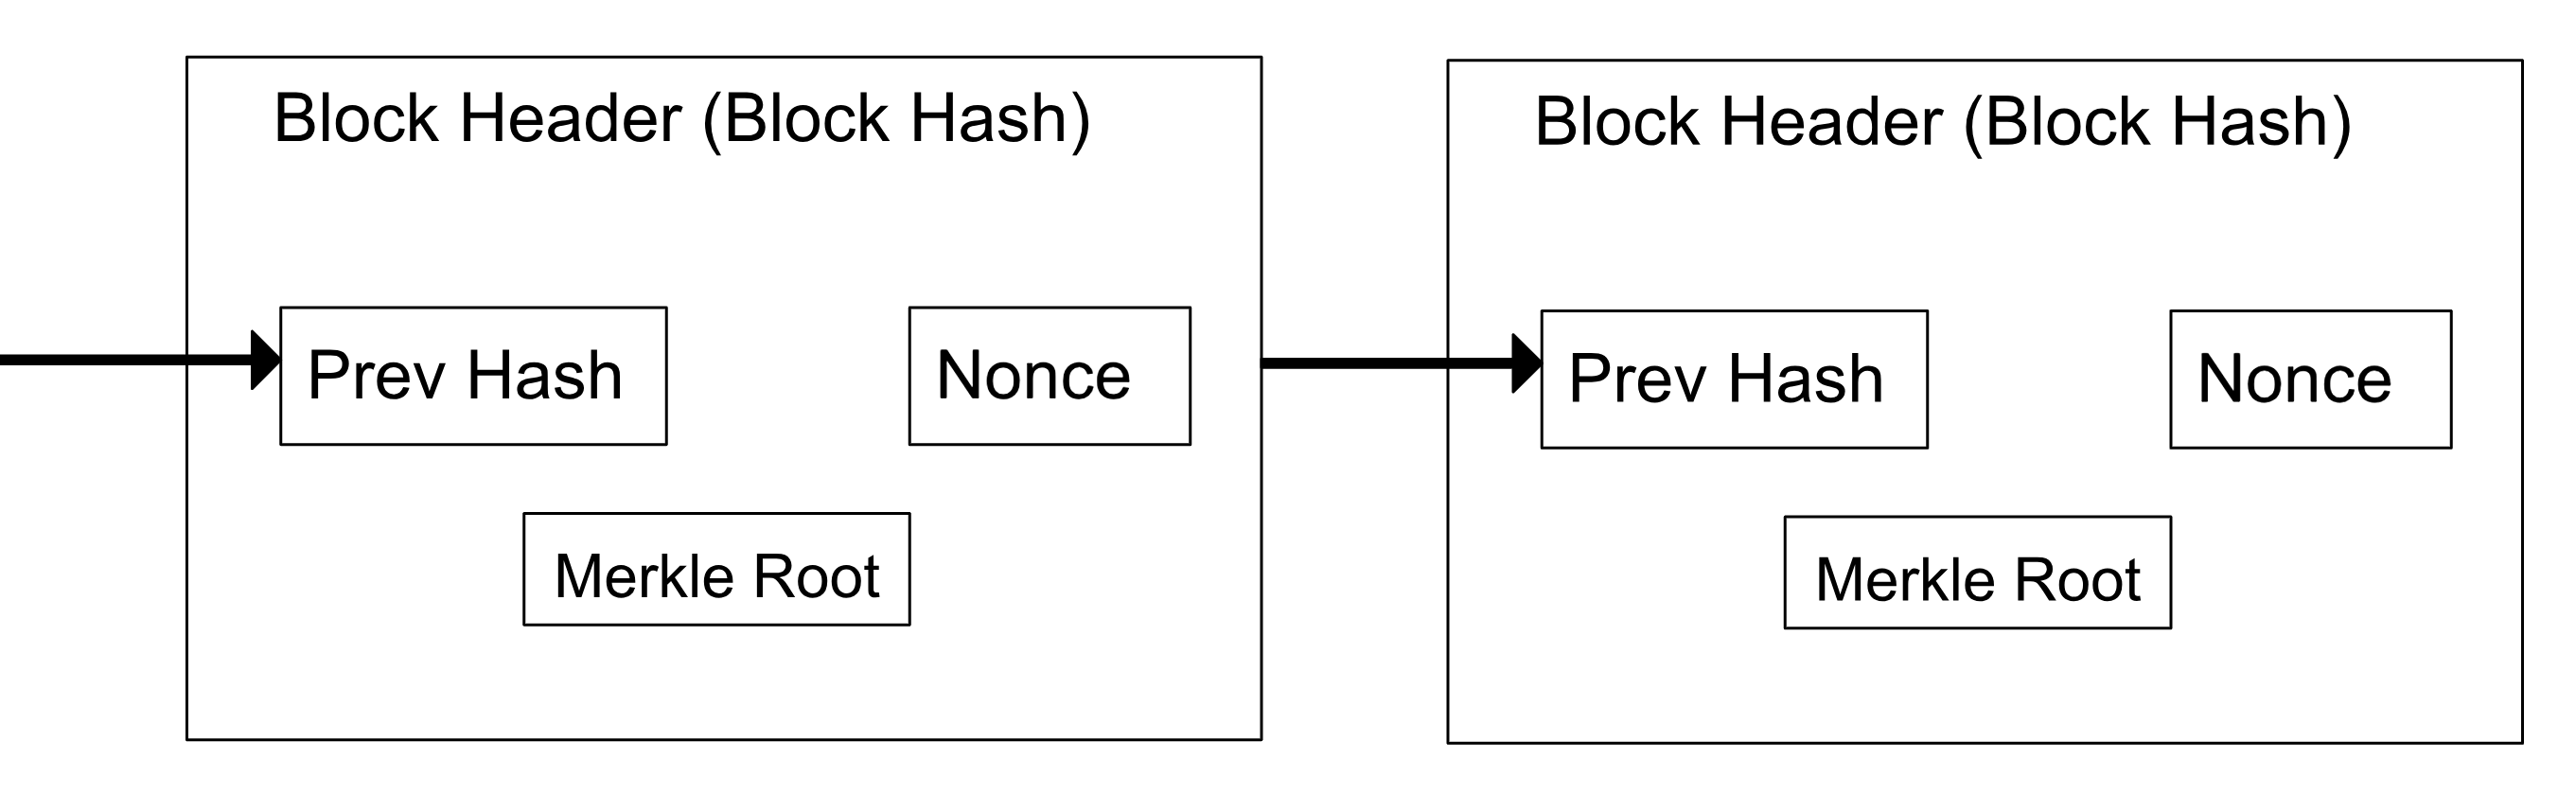
\includegraphics[width=.45\textwidth]{graphics/blocks_merkle.png}
  \caption{Bitcoin blocks with merkle root}
  \label{fig:fig6}
\end{figure}

Figure 7 displays how Merkle tree is constructed with four transactions.

\begin{figure}[h]
  \centering
  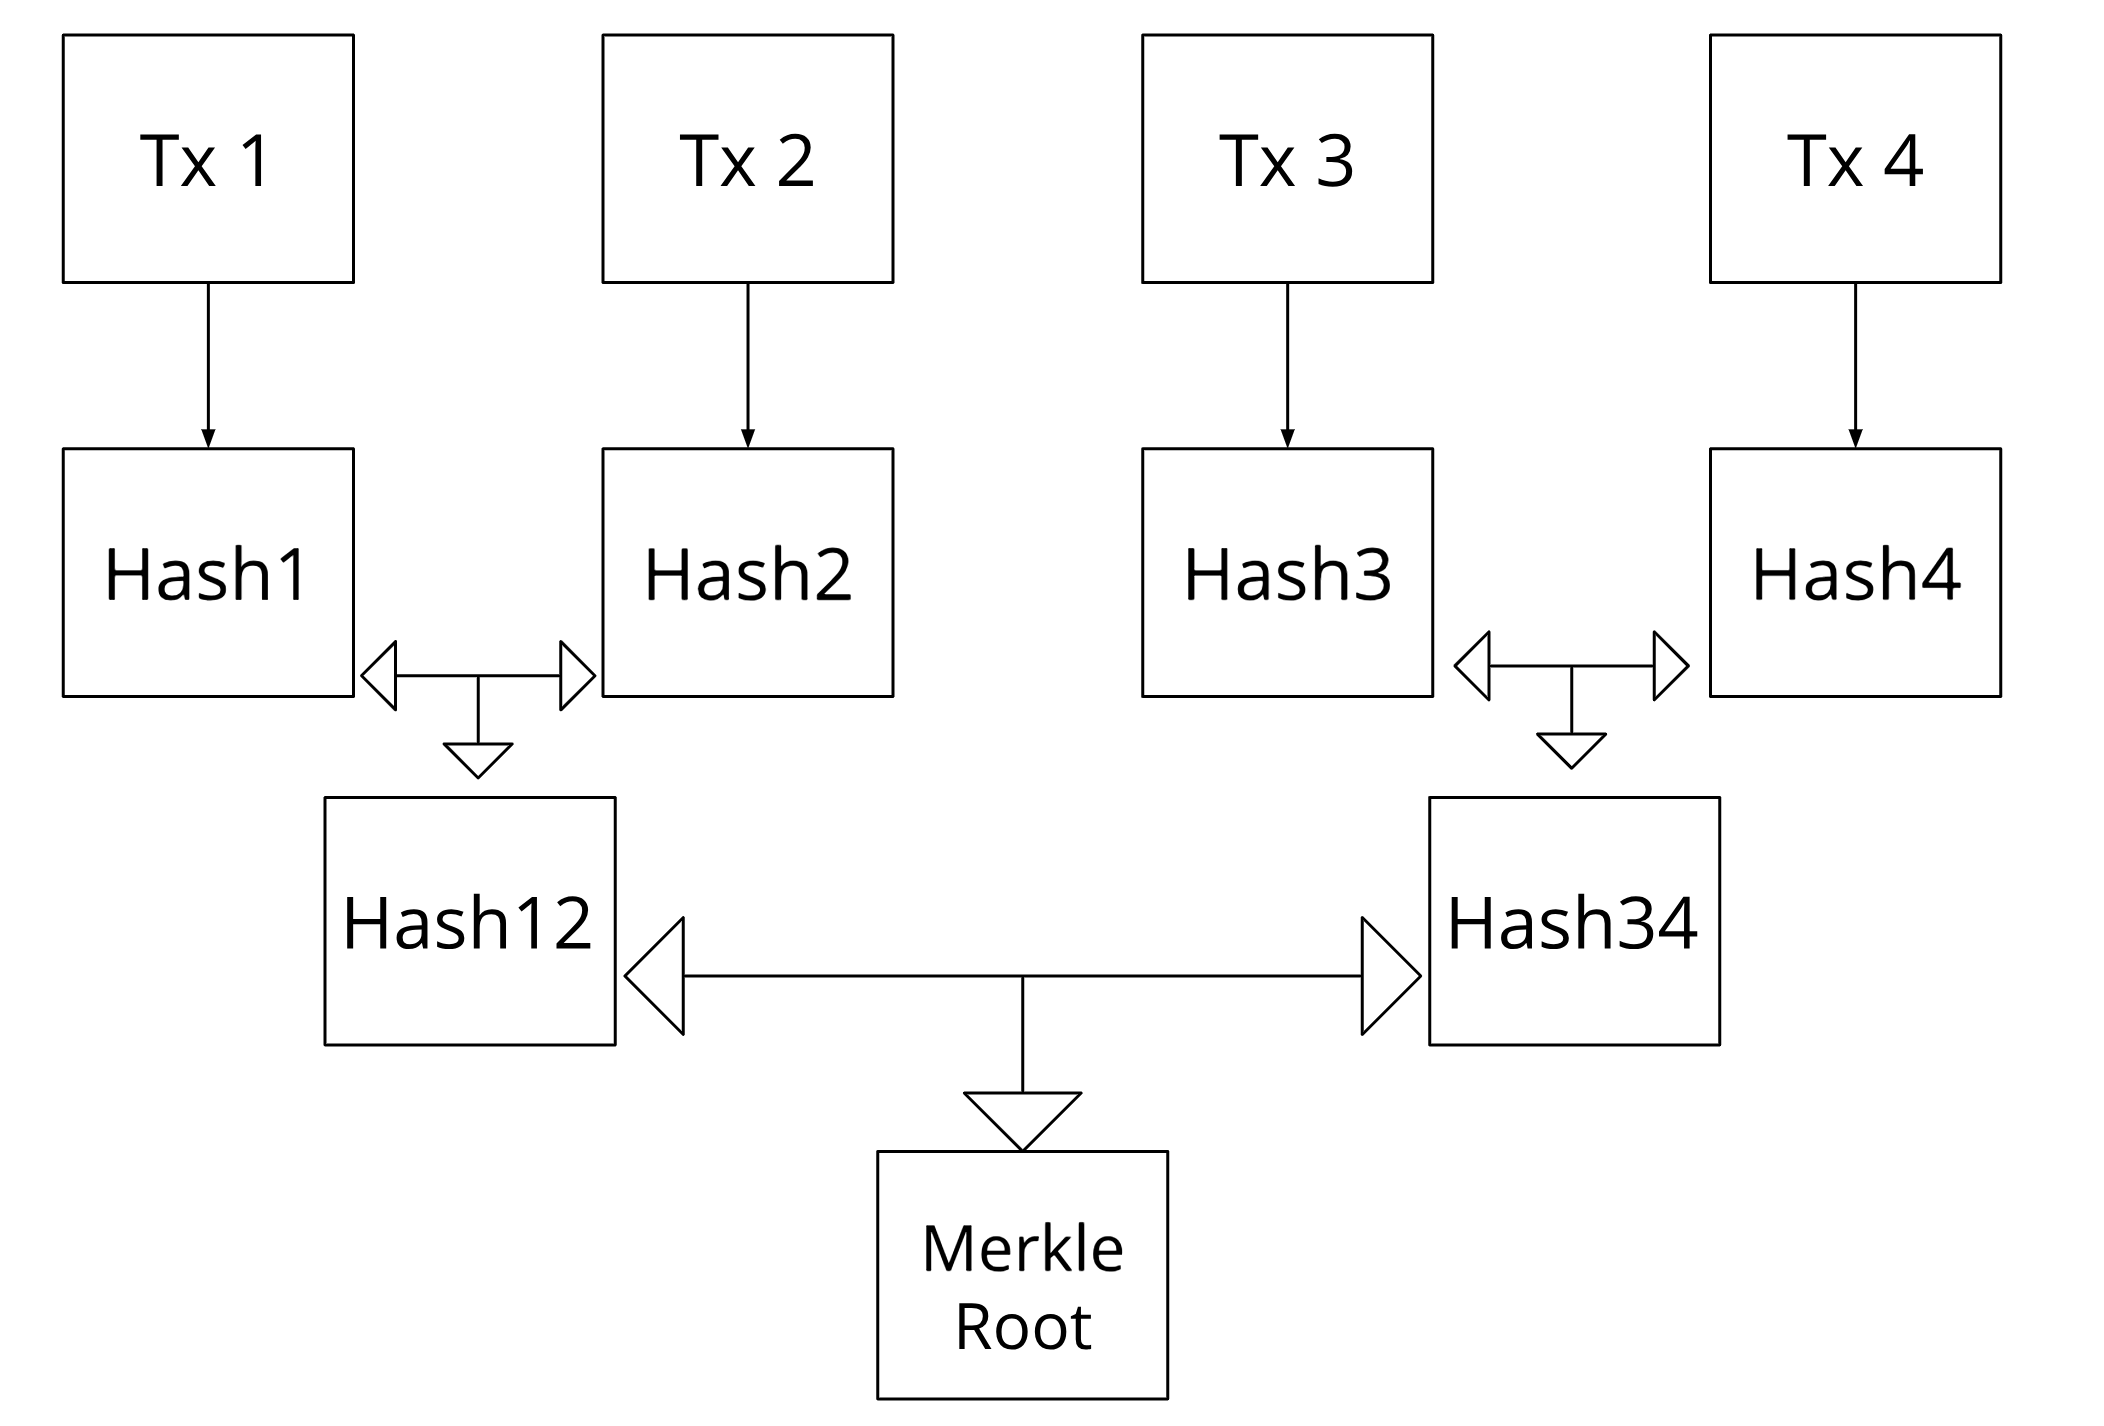
\includegraphics[width=.45\textwidth]{graphics/merkle.png}
  \caption{Merkle Tree}
  \label{fig:fig7}
\end{figure}

\subsubsection{Bitcoin: creation and reward}
It is not a secret that government is responsible for printing new money into the financial system. 
At least, it is true for traditional fiat currencies.
But Bitcoin is fundamentally different in a sense that there is no central authority.
So how new bitcoins are created?
The process of issuing new coins tied closely to mining mechanism. 
In order to make nodes spend their computational resources on mining new blocks, network adds special transaction to a block. 
This transaction is addressed to a node that successfully mined a block and contains a reward. 
In other words, reward is way for a network to issue new coins into the system. 
However, bitcoin is deflationary currency. 
It means that there is finite number of bitcoins that will be created. 
It is achieved by reducing reward in half roughly every four years. 
Here is timeline showing how it works:

\begin{itemize}
    \item 01.2009 - 10.2012: 50 BTC
    \item 10.2012 - 07.2016: 25 BTC
    \item 07.2016 - 02.2020: 12.5 BTC (current reward)
    \item 02.2020 - 09.2023: 6.25 BTC
    \item ...
\end{itemize}

It is calculated that in total there will be no more that twenty one million of bitcoins. 
Possibly even less, due to the fact that if private key for the wallet is lost, all associated bitcoins are also gone forever. 

But what will be incentive for miners to keep working after reward is really small or equals to zero? 
Well, it is known that each transaction can have at most two outputs: one for recipient, one for returning the change. 
But if second output is not specified and input value is greater than output, then the difference is counted as a transaction fee and it goes to the block miner.


\section{Conclusion}
The conclusion goes here.




% conference papers do not normally have an appendix



% use section* for acknowledgment
\ifCLASSOPTIONcompsoc
  % The Computer Society usually uses the plural form
  \section*{Acknowledgments}
\else
  % regular IEEE prefers the singular form
  \section*{Acknowledgment}
\fi


The authors would like to thank...





% trigger a \newpage just before the given reference
% number - used to balance the columns on the last page
% adjust value as needed - may need to be readjusted if
% the document is modified later
%\IEEEtriggeratref{8}
% The "triggered" command can be changed if desired:
%\IEEEtriggercmd{\enlargethispage{-5in}}

% references section

% can use a bibliography generated by BibTeX as a .bbl file
% BibTeX documentation can be easily obtained at:
% http://mirror.ctan.org/biblio/bibtex/contrib/doc/
% The IEEEtran BibTeX style support page is at:
% http://www.michaelshell.org/tex/ieeetran/bibtex/
%\bibliographystyle{IEEEtran}
% argument is your BibTeX string definitions and bibliography database(s)
%\bibliography{IEEEabrv,../bib/paper}
%
% <OR> manually copy in the resultant .bbl file
% set second argument of \begin to the number of references
% (used to reserve space for the reference number labels box)
\begin{thebibliography}{1}

\bibitem{IEEEhowto:kopka}
H.~Kopka and P.~W. Daly, \emph{A Guide to \LaTeX}, 3rd~ed.\hskip 1em plus
  0.5em minus 0.4em\relax Harlow, England: Addison-Wesley, 1999.

\end{thebibliography}




% that's all folks
\end{document}


